%%%%%%%%%%%%%%%%%%%%%%%%%%%%%%%%%%%%%%%%%%%%%%%%%%%%%%%%%%%%%%%%%%%%%%%%%%%%
%
%		Relazione sul Dead Reckoning - Peer 2 Peer
%
%				    Nicola Corti - 2013
%
%%%%%%%%%%%%%%%%%%%%%%%%%%%%%%%%%%%%%%%%%%%%%%%%%%%%%%%%%%%%%%%%%%%%%%%%%%5%
\documentclass[a4paper,11pt]{article} 
\usepackage{graphicx}
\usepackage{vmargin}
\usepackage[italian]{babel} 
\usepackage[utf8x]{inputenc}
\usepackage{listings}
\usepackage{url}
\usepackage{pdflscape}
\usepackage{hyperref}
\usepackage{indentfirst}
\usepackage{tabularx}
\usepackage{bm}
\usepackage{amsmath}
\usepackage{subfigure}
\usepackage[usenames,dvipsnames,svgnames,table]{xcolor}

\newcolumntype{P}[1]{>{\raggedright\arraybackslash}p{#1}}

\lstset{
basicstyle=\small\ttfamily,
keywordstyle=\color{MidnightBlue}\bfseries,
identifierstyle=\color{Black},
commentstyle=\color{Green}\itshape,
stringstyle=\color{Red}\ttfamily,
showstringspaces=false,
%numbers=left, numberstyle=\tiny,
%stepnumber=1, numbersep=10pt,
tabsize=4,
framexleftmargin=5mm, rulesepcolor=\color{Gray},
frame=tb,
backgroundcolor=\color{LightGray},
language={Java},
%mathescape=true,
%fontadjust=true,
%breaklines=true,breakatwhitespace=true,breakautoindent
}


\title{\emph{Dead Reckoning} - Meccanismi per compensare la mancanza di risorse nei Multiplayer Mass Online Games}
\author{Nicola Corti - 454413 \\Corso di Laurea Magistrale in Informatica - Universit\`a di pisa}
\date{10 Dicembre 2013}

\renewcommand\lstlistingname{Codice}
\renewcommand\figurename{Immagine}
 
\begin{document}
\maketitle
 
\begin{abstract}
Questa relazione ha lo scopo di presentare il meccanismo del \emph{Dead Reckoning}, meccanismo largamente utilizzato nel campo dei MMOG (Multiplayer Mass Online Games) per ridurre i ritardi del gioco generati dalla latenza di comunicazione della rete. Verranno dapprima presentate le metodologie base, con i vari benefici ed le varie difficolt\`a che si possono incontrare utilizzando il \emph{Dead Reckoning}, e successivamente verranno analizzate alcune alternative ed evoluzioni proposte al sistema del \emph{Dead Reckoning}.
\end{abstract}

\tableofcontents

\section*{Introduzione}

Fra tutti software che sono stati mai realizzati dall'industria informatica, forse i pi\`u complessi che si possano pensare sono i videogame.

Per poter realizzare un videogames \`e infatti necessario avere competenze che toccano tutti gli aspetti dell'informatica, dalla grafica tridimensionale in primis, ai database, senza ovviamente escludere l'intelligenza artificiale.

Il mercato videoludico, nato negli anni '70 con il primo \emph{Pong}\footnote{\url{http://en.wikipedia.org/wiki/Pong}} o altri giochi dello stesso calibro, ha subito fino ad oggi notevoli impennate fino ad invadere la vita di tutte le persone, con console presenti nella casa di molte persone e videogiochi che possono essere fruiti facilmente e gratuitamente tramite ogni tipo di piattaforma.

A fare da padrone a questa crescita \`e stato probabilmente l'introduzione di un'altra tecnologia all'interno dello sviluppo dei videogiochi: il networking. A partire dagli anni '90 sono nati i primi MMORPGs (Multiplayer Mass Online Role Play Games \cite{wiki1}), giochi di ruolo multigiocatore quali \emph{Ultima Online}\footnote{\url{http://www.uo.com/}}, \emph{Lineage}\footnote{\url{http://lineage.plaync.com/}} o \emph{EverQuest}\footnote{\url{https://www.everquest.com/}} che sono riusciti ad unire alla componente videoludica una componente multiplayer, permettendo ai videogiocatori di incontrarsi e di scontrarsi attraverso la rete, offrendo un livello di sfida ovviamente non raggiungibile dai personaggi gestiti dalla CPU.

Attualmente il mercato MMOG \`e considerato uno fra i mercati pi\`u importante in campo videoludico, con giochi quali \emph{World of Warcraft}\footnote{\url{http://battle.net/wow/}}(sviluppato da Blizzard - figura \ref{img:wow}) o \emph{League of Legends}\footnote{\url{http://leagueoflegends.com/}}(sviluppato da Riot) che toccano picchi di 30 milioni di videogiocatori connessi al mese (di cui una media di 10 milioni di videogiocatori connessi contemporaneamente)\footnote{\href{http://www.gamesindustry.biz/articles/2012-10-12-league-of-legends-32-million-monthly-active-users}{Game Industry - League of Legends: 32 million monthly active players\small}}.

\begin{figure}[ht]
\centering
\includegraphics[height=6cm]{wow.jpeg}
\caption{\small{Screenshot tratto dal videogioco World of Warcraft - Si possono notare i personaggi di tutti i giocatori collegati}}
\label{img:wow}
\end{figure}

Ovviamente l'introduzione del networking all'interno dei videogiochi ha portato con se notevoli criticit\`a che devono essere prese in considerazione durante lo sviluppo del software e durante la realizzazione dell'infrastruttura che possa supportare un tale carico. Si consideri inoltre che questi software richiedono un numero molto elevato di risorse: potenza di calcolo e memoria per effettuare il rendering 3D del mondo di gioco, spazio disco per memorizzare mappe, mondi, video ed altro materiale multimediale, banda di rete per effettuare la comunicazione con il server e con gli altri giocatori.

In particolare la banda e la latenza della rete possono molto spesso diventare dei \emph{bottleneck} e rallentare il gioco, si consideri infatti che possono connettersi a giocare persone geograficamente dislocate in luoghi molto distanti del globo. Il software deve occuparsi di gestire questi problemi, al fine di offrire un'esperienza di gioco che non sia affetta da ritardi, che potrebbero altrimenti rendere l'esperienza talmente pessima, tanto da rendere il gioco ingiocabile, con conseguente perdita della clientela da parte della software house produttrice.

Fra i vari meccanismi sviluppati per gestire questi ritardi, uno fra i pi\`u utilizzati \`e il \emph{Dead Reckoning} che si occupa sostanzialmente di prevedere gli spostamenti dei giocatori in base ai loro precedenti spostamenti, prendendo in considerazione informazioni quale la posizione, la velocit\`a e l'accelerazione.

\section{Il fenomeno del \emph{Lag}}

Il compito del server che gestisce un MMOG \`e quello di:
\begin{itemize}
\item Mantenere lo stato del gioco consistente,
\item Ricevere e gestire gli eventi provenienti dagli utenti e modificare lo stato di conseguenza.
\end{itemize}

Lo stato del gioco e gli eventi da gestire variano ovviamente in base al tipo di gioco come descritto nella tabella \ref{tab:stati}.

\begin{table}[h]
\label{tab:stati}
\centering
\begin{tabular}{|P{3.20cm}|P{5cm}|P{5cm}|}
\hline
\textbf{Tipo di gioco} & \textbf{Esempi di stato} & \textbf{Esempi di Eventi} \\
\hline
FPS (\emph{First Person Shooter}) & Posizione degli altri giocatori e dei power-up sulla mappa & Spostamento dei giocatori e sparo di un colpo  \\
\hline
RTS (\emph{Real Time Strategy}) & Posizione delle truppe, degli edifici e delle risorse & Spostamento delle truppe ed attacchi fra truppe  \\
\hline
RPG (\emph{Role Play Game}) & Posizione del proprio avatar, dei mostri e degli avatar degli altri giocatori & Spostamento dell'avatar, uso o raccolta di un oggetto, attacco di un mostro o di un altro avatar, interazione con gli altri avatar (chat, etc...)  \\
\hline
Simulazione & Posizione del proprio veicolo (aereo, macchina, etc...) e posizione dei veicoli avversari & Cambiamento della velocit\`a e della direzione del veicolo  \\
\hline
Sportivo & Posizione del proprio personaggio e dei personaggi avversari & Cambiamento di posizione, passaggi di palla, tiri, altre azioni dipendenti dallo sport.  \\
\hline
\end{tabular}
\caption{\small{Tipi di gioco con esempi di stato e di eventi da gestire}}
\end{table}

Le comunicazioni fra i client dei giocatori e il server di gioco avvengono attraverso la rete, sia essa una rete LAN oppure Internet, che introduce dei ritardi, in parte generati dal fatto che la larghezza di banda dei client \`e limitata, ed in parte generati dal fatto che \`e presente una latenza di comunicazione fra il server e il client (dovuto ai vari router che ogni pacchetto deve attraversare per raggiungere il server). La latenza di comunicazione fra il server e il client viene chiamata anche \emph{Ping}.

Se consideriamo lo scenario delle connessioni attuale, la larghezza di banda \`e diventata sufficientemente ampia (molti utenti riescono infatti a connettersi tramite connessioni ADSL ad elevate velocit\`a) da non creare rallentamenti significativi, mentre invece esistono latenze di comunicazione che possono generare ritardi notevoli (si pensi ad esempio alla latenza di comunicazione fra Europa ed America oppure fra Europa ed Asia).

Inoltre i ritardi possono essere amplificati dal fenomento della pardita di pacchetti (\emph{packet loss}) oppure dal fatto di utilizzare macchine con potenza di calcolo ridotta, che tardano nell'inviare e nel ricevere i pacchetti.

Nel caso in cui il ritardo di comunicazione complessivo fra il client e il server risulti troppo alto \`e possibile che il server non riesca pi\`u a mantenere lo stato consistente, gli eventi generati dai client possono essere ricevuti in ritardo e non nell'ordine temporale in cui erano stati effettivamente generati dai client. Il server deve quindi affrontare questa situazione e riportare lo stato ad una situazione consistente.

Si verifica quello che viene appellato dai videogiocatori come \emph{Lag} (\cite{wiki2} - dall'inglese ritardo oppure \emph{Latency GAp}), i videogiocatori possono notare personaggi che si muovono a scatti, personaggi che non si muovono e possono addirittura non riuscire pi\`u a controllare l'intero gioco. L'esperienza del \emph{Lag} pu\`o essere talmente frustrante da portare il giocatore a cambiare videogioco e si deve quindi cercare di evitarla per quanto possibile.

%%%%%%%%%%
% GRAFICO RICCI
%%%%%%%%%%


\section{Il \emph{Dead Reckoning}}

Il \emph{Dead Reckoning} (\cite{rif1}) \`e un meccanismo per mitigare i ritardi introdotti dalla rete al fine di evitare il manifestarsi dei \emph{Lag} e rendere l'esperienza utente pi\`u fluida.

Un sistema che non utilizza il \emph{Dead Reckoning} obbliga i client ad inviare tutti i cambiamenti di posizione dell'avatar del giocatore con una frequenza molto elevata. Utilizzando invece il \emph{Dead Reckoning} \`e possibile diminuire la frequenza con cui vengono inviati i messaggi dal client al server, i messaggi inviati contengono per\`o informazioni ulteriori oltre alla semplice posizione quali ad esempio la velocit\`a (modulo, direzione e verso) e l'accelerazione (modulo, direzione e verso). Utilizzando queste informazioni e le leggi fisiche della cinematica \`e possibile prevedere gli spostamenti degli altri giocatori.

Utilizzando questo sistema il client invia un nuovo messaggio solamente quando effettua degli spostamenti significativi, oppure quando varia la velocit\`a e l'accelerazione, riducendo quindi notevolmente il carico complessivo del traffico in entrata al server e comportando un significativo miglioramento delle performance (\cite{rif2}).

Questa fase del meccanismo di \emph{Dead Reckoning} viene detta fase di \emph{Prediction}, in base al fatto che si cerca di prevedere dove si trover\`a il giocatore partendo dai dati ricevuti.

Nel caso in cui la posizione predetta si discosti dalla posizione effettiva ricevuta successivamente \`e necessario effettuare una correzione della posizione del personaggio: questa fase prende il nome di \emph{Convergence} e deve essere realizzata nel modo pi\`u gradevole possibile per l'utente.

\begin{figure}[ht]
\centering
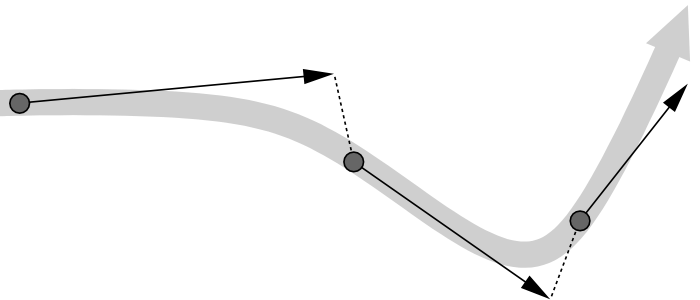
\includegraphics[height=3cm]{dr.png}
\caption{\small{Esempio di utilizzo del meccanismo del \emph{Dead Reckoning}, in grigio \`e rappresentato il movimento del giocatore, i cerchi rappresentano le posizioni con i vettori velocit\`a (le frecce) inviate ad ogni messaggio. Le linee tratteggiate rappresentano gli spostamenti di posizione che devono essere gestiti nella fase di convergence.}}
\label{img:dr}
\end{figure}

\subsection{Fase di \emph{Prediction}}

La fase di prediction consiste fondamentalmente nella predizione della posizione a partire dai dati ricevuti. Generalmente, oltre alla posizione del personaggio, si implementa la prediction utilizzando la velocit\`a e l'accelerazione. In particolare consideriamo la velocit\`a e l'accelerazione rispettivamente come la derivata prima e seconda della posizione rispetto al tempo; risulta cruciale la decisione dell'approssimazione da utilizzare, un'approssimazione al primo ordine che prende in considerazione solo la velocit\`a, un'approssimazione del secondo ordine che prende in considerazione velocit\`a ed accelerazione, oppure un'approssimazione di ordine superiore.

Utilizzando velocit\`a ed accelerazione \`e possibile anche determinare quando il client deve inviare un nuovo messaggio: \`e sufficiente determinare un valore di soglia da confrontare con la variazione di velocit\`a ed accelerazione: nel caso in cui la variazione sia superiore alla soglia il client invier\`a un nuovo messaggio, altrimenti la piccola variazione risulta tollerabile e non va ad impattare sul gioco.



\paragraph{Predizione utilizzando approssimazione al primo ordine}

La predizione con approssimazione al primo ordine prende in considerazione solamente la velocit\`a e calcola la nuova posizione utilizzando la seguente legge della cinematica: $$ p(t) = p(0) + v(0) t$$

Dove $p(t)$ rappresenta la posizione al tempo $t$ e $v(t)$ rappresenta la velocit\`a al tempo $t$.

Si potrebbe essere portati a pensare che un'approssimazione di secondo ordine, malgrado sia pi\`u onerosa dal punto di vista computazionale, possa offrire dei risultati migliori in termini di precisione, ma non \`e sempre cos\`i.

Un discorso del genere pu\`o valere per videogiochi di simulazione dove l'accelerazione non varia molto, ma pu\`o portare a risultati fuorvianti nel caso di giochi RTS, FPS o RPG: in questi giochi i giocatori possono effettuare repentini cambi di direzione e l'accelerazione pu\`o portare a predizioni molto distanti dalla realt\`a. 

\paragraph{Predizione utilizzando approssimazione la secondo ordine}

La predizione con approssimazione al primo ordine prende in considerazione anche l'accelerazione e calcola la nuova posizione utilizzando la seguente legge della cinematica: $$ p(t) = p(0) + v(0)\cdot t + \frac{1}{2} a(0) t^2 $$

Dove $p(t)$ rappresenta la posizione al tempo $t$, $v(t)$ rappresenta la velocit\`a al tempo $t$ e $a(t)$ rappresenta l'accelerazione al tempo $t$. Si noti come il termine dell'accelerazione consideri il tempo al quadrato per cui piccoli errori nell'accelerazione possono portare a grosse differenze nella posizione.

Questo genere di approssimazione \`e dunque utilizzata per i videogiochi dove l'accelerazione non varia troppo: ad esempio nei giochi di simulazione di veicoli.

\paragraph{Predizione utilizzando approssimazione di ordini superiori}

Le predizioni di ordine superiore (quelle che prendono in considerazione gli \emph{strappi}) vengono spesso scartate in quanto introducono errori maggiori a quelle del secondo ordine e risultano inoltre molto difficili da calcolare, in quanto molto spesso l'accelerazione varia in base alle decisioni dell'utente e risulta difficile da prevedere.


\subsection{Fase di \emph{Convergence}}

Nella fase di prediction vengono quindi calcolate le nuove posizioni assunte dal personaggio, considerando i dati ricevuti dal client in ogni messaggio. Nel caso in cui la posizione ricevuta dal client sia troppo distante dalla posizione predetta \`e necessario correggere questa discrepanza: ha dunque luogo la fase di convergence.

La fase di convergence consiste fondamentalmente nel riposizionamento del giocatore, in modo da correggere l'errore generato dalla previsione. Questo riposizionamento pu\`o essere effettuata in svariati modi, pi\`u o meno gradevoli (immagine \ref{img:conv}).

\begin{figure}[ht]
\centering
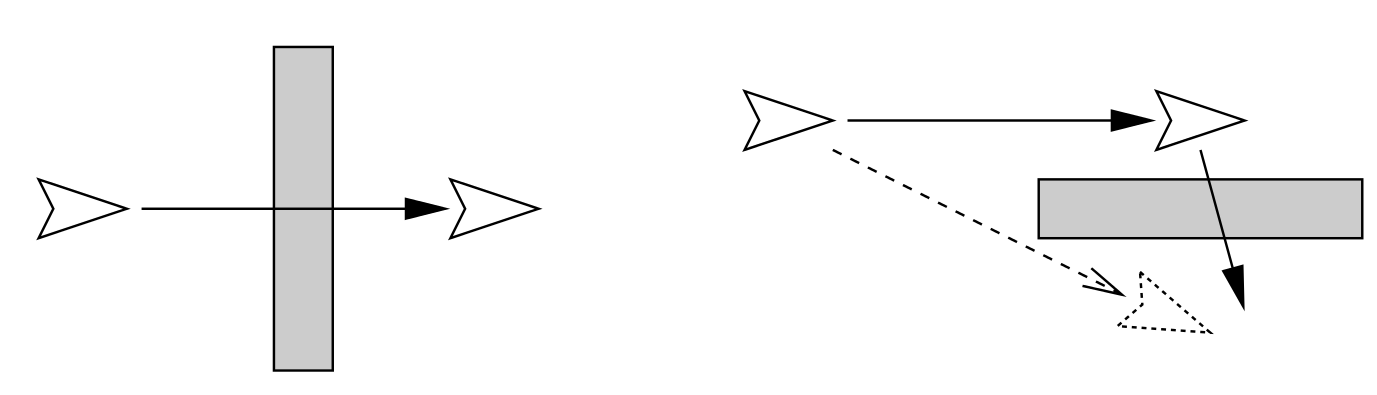
\includegraphics[height=2.5cm]{conv.png}
\caption{\small{Esempio di utilizzo del meccanismo di \emph{convergence}, nell'immagine di sinistra si usa la versione \emph{snap} mentre nell'immagine di destra si usa la versione lineare}}
\label{img:conv}
\end{figure}


\paragraph{Convergenza tramite \emph{Snap}}

La convergenza tramite \emph{snap} consiste semplicemente nel riposizionare il giocatore alla nuova posizione, senza effettuare posizionamenti intermedi.

Questa tecnica risulta la pi\`u semplice da implementare, ma al contempo \`e anche quella pi\`u sgradevole per l'utente, dato che il giocatore non vede il personaggio che si ``teletrasporta'' fra un punto ed un altro, senza percorrere alcun percorso; si avr\`a quindi una forte percezione del lag che potrebbe inficiare l'esperienza di gioco.

Per questo motivo si cerca di implementare quantomeno una convergenza di tipo lineare, per rendere meno sgradevole l'evento.

\paragraph{Convergenza Lineare}

La convergenza lineare consiste in realizzare un'interpolazione lineare fra il punto di partenza e il nuovo punto. Cos\`i facendo il giocatore ha la percezione che il personaggio si stia muovendo lungo una linea retta.

Per la convergenza lineare \`e possibile ad esempio utilizzare la formula seguente: sia $s_1$ la posizione al tempo $t_1$ e sia $s_2$ la posizione al tempo $t_2$, si vuole calcolare la posizione $s$ al tempo $t$ con $t_1 < t < t_2$:

$$ s = \frac{(t - t_1)}{(t_2 - t_1)} \cdot (s_2 - s_1) + s_1 $$

La convergenza lineare \`e da preferirsi a quella di tipo \emph{snap}, anche se pu\`o portare a percorsi che possono comunque risultare innaturali. L'utente non si aspetta infatti che tutti i personaggi si muovano lungo linee rette, ma si aspetta movimenti che siano lungo linee curve (quella che viene chiamo un percorso di tipo \emph{smooth}), per questo si pu\`o ricorrere alle convergenze di ordine superiore.

\paragraph{Convergenza di ordine superiore}

La convergenza di ordine superiore permette di ottenere curve che siano pi\`u dolci di una semplice linea retta. Per utilizzare questo meccanismo si pu\`o ricorrere a curve di tipo differente, una curva di tipo famoso \`e la curva di B\'ezier cubica.

In particolare assumiamo che $s_1$ sia la posizione al tempo $t_1$, e sia $s_2$ la posizione al tempo $t_2$, consideriamo $\bar{s_1}$, $\bar{t_1}$, $\bar{s_2}$ e $\bar{t_2}$ le predizioni a partire da $s_1$ e da $s_2$ con i loro relativi tempi, \`e possibile creare una curva di B\'ezier che unisce i punti $s_1$ e $\bar{s_2}$ usando la formula seguente:

$$ s(t') = s_1(1 - t')^3 + 3 \cdot \bar{s_1} t' (1 - t')^2 + 3 \cdot s_2 t^2(1 - t') + \bar{s_2}t'^3 \qquad t' = \frac{(t - t_1)}{(\bar{t_2} - t_1)}$$

Con $t_1 < t' < \bar{t_2}$.

\begin{figure}[ht]
\centering
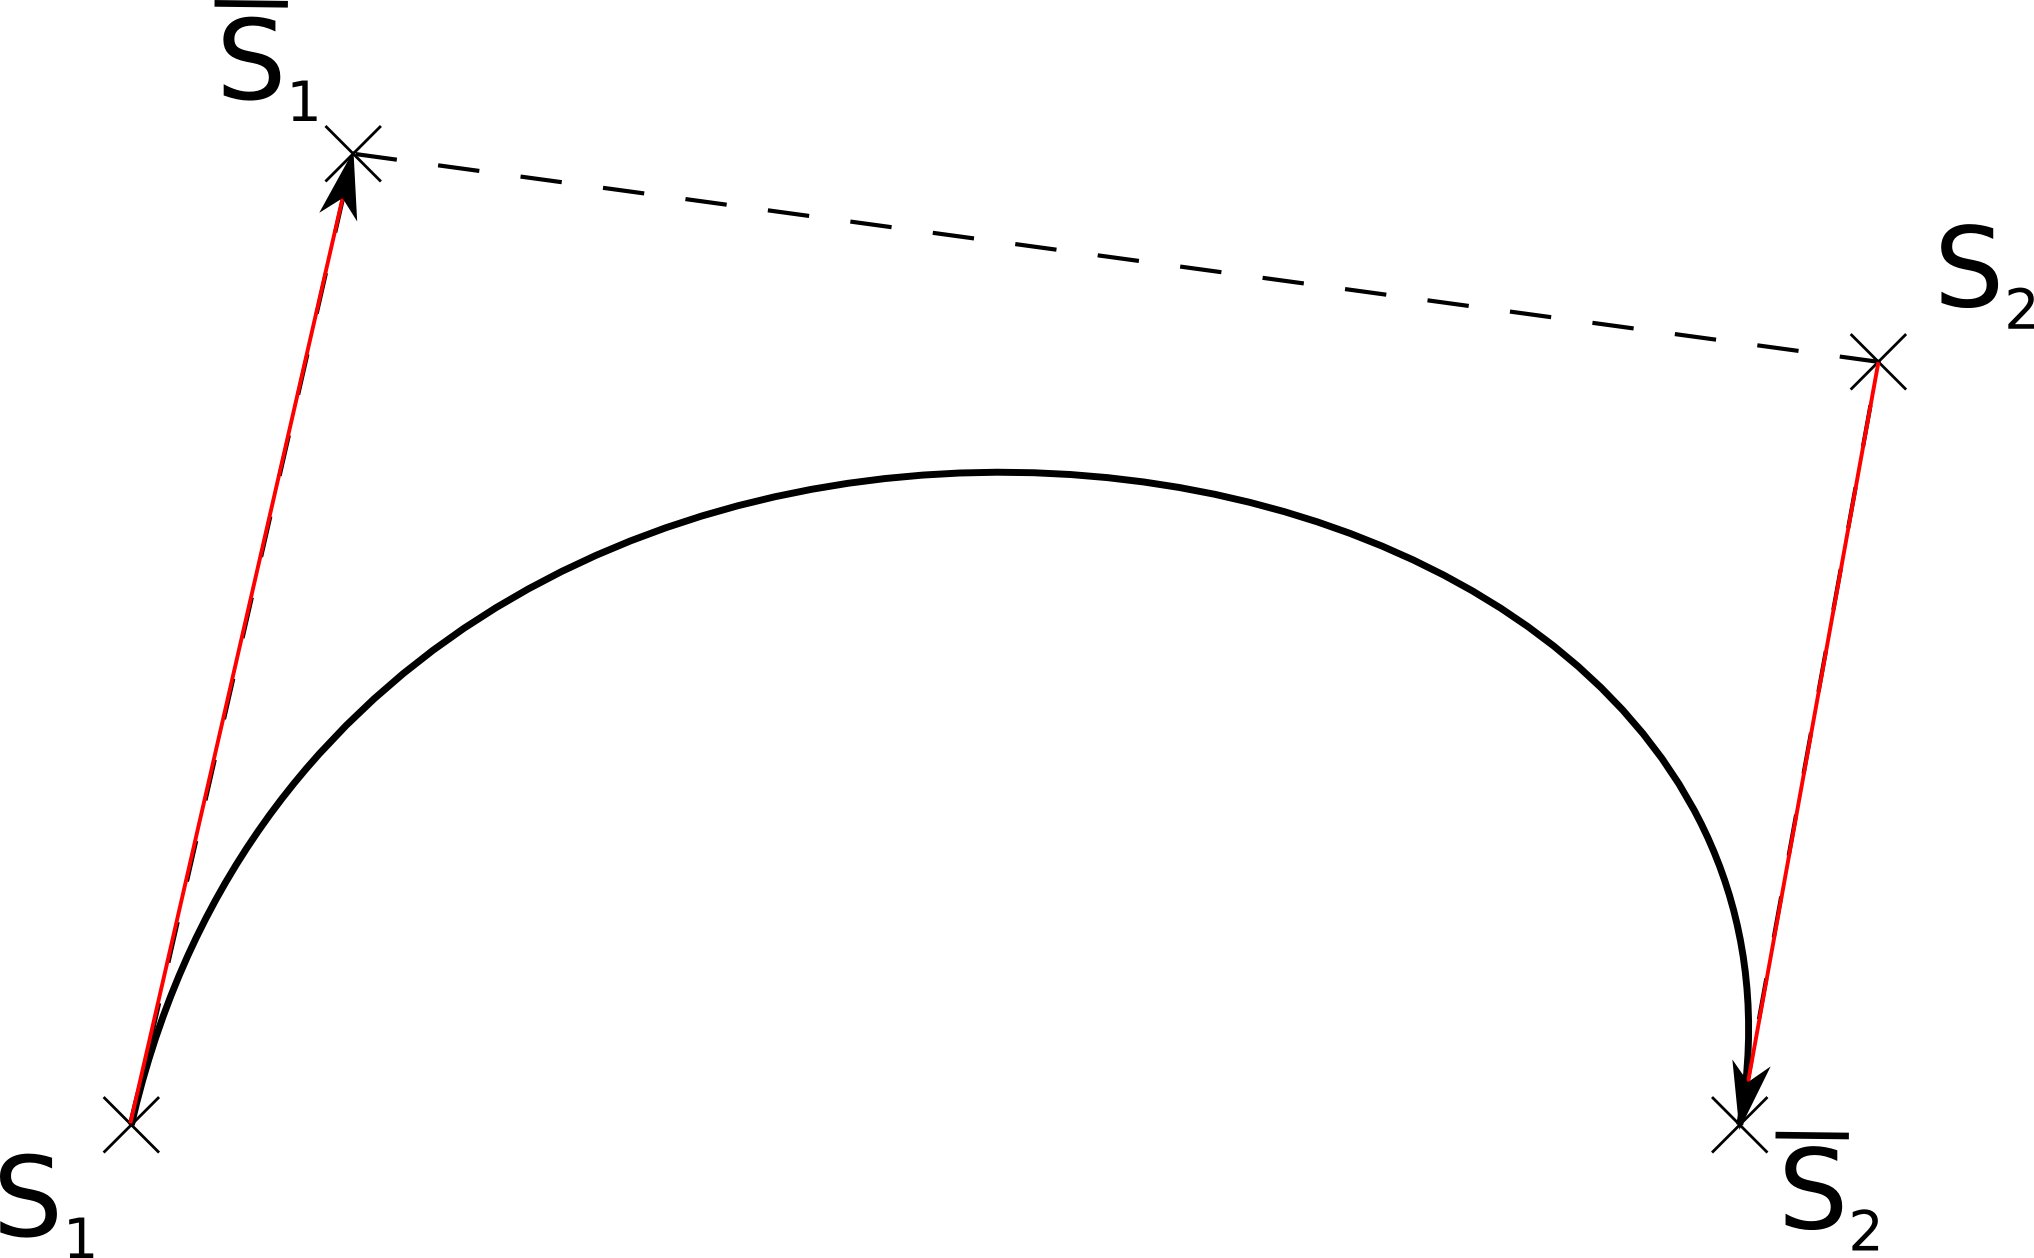
\includegraphics[height=5cm]{bez.png}
\caption{\small{Esempio di percorso generato dalla \emph{convergence} con curva di bezier quadratica fra i punti $s_1$ e $s_2$ e le loro relative predizioni $\bar{s_1}$ e $\bar{s_2}$}}
\label{img:bez}
\end{figure}

Questa curva offre una convergenza migliore di quella lineare (immagine \ref{img:bez}), ma pu\`o portare a computazioni pi\`u complesse in quanto sono presenti termini al quadrato e al cubo che possono rallentare il calcolo.

\section{Inconsistenza dello stato}

Sebbene l'utilizzo del \emph{Dead Reckoning} riduca notevolmente il carico di rete, non si \`e preso in considerazione ci\`o che accade se i pacchetti che contengono le informazioni di velocit\`a ed accelerazione vengono persi.

Il sistema del \emph{Dead Reckoning} gode fortunatamente della propriet\`a del \emph{Self-healing}: nel caso in cui un pacchetto venga perso oppure che subisca un grosso delay, verr\`a effettuata la convergenza utilizzando il pacchetto successivo e il sistema del \emph{Dead Reckoning} continuer\`a a funzionare.

Purtroppo questo meccanismo, malgrado sia robusto, non tiene in considerazione il fatto che pu\`o portare lo stato di gioco ad una situazione di inconsistenza, si consideri l'esempio seguente:

\paragraph{A Dead Man that Shoots}

Si supponga che il giocatore A spari un colpo di proiettile verso il giocatore B. Ovviamente il client memorizza velocit\`a ed accelerazione del proiettile e li invia al server.

Purtroppo il pacchetto contente questi dati subisce un forte delay a causa dell'infrastruttura di rete; nel mentre il giocatore B spara un colpo verso il giocatore C. Il pacchetto contenente queste informazioni non viene rallentato a causa dell'infrastruttura di rete di B (che risulta essere meno affetta da ritardi rispetto a quella di A) e arriva al server provocando la morte di C.

Il pacchetto contente la pallottola sparata di A arriva in un secondo momento al server e provoca la morte di B.

\subsection{Utilizzo dei \emph{timewarp}}

Per sopperire a questo problema \`e necessario definire un ordinamento fra gli eventi che sono stati registrati dai client, in modo da poterli eseguire in modo ordinato e a non portare ad un'inconsistenza dello stato (\cite{rif3}, \cite{rif4}).

Ci\`o \`e possibile utilizzando dei \emph{timestamps}, cio\`e corredando l'informazione sulla velocit\`a e sull'accelerazione di una marca temporale che indichi il tempo a cui \`e stata generato l'evento. Ci\`o \`e possibile utilizzando un protocollo quale NTP\footnote{RFC 958 - \url{http://tools.ietf.org/html/rfc958}} (Network Time Protocol), che permette di sincronizzare l'orologio dei client al fine di avere un ordinamento temporale degli eventi.

Utilizzando questa informazione ulteriore \`e quindi possibile utilizzare un algoritmo che si basa sui \emph{timewarp}: ogni client invia i propri eventi a tutti gli altri client aggiungendo i dati sul tempo in cui \`e stato generato l'evento; i client memorizzano tutti gli eventi che hanno ricevuto in ordine cronologico ed effettuano dei \emph{timewarp} alla ricezione di nuovi eventi, ovvero ricalcolano lo stato eseguendo in ordine gli eventi che hanno ricevuto.

In questo modo tutti i client si ``accordano'' sullo stato effettivo e non si genera inconsistenza, in particolare nel caso del \emph{Dead Man that Shoots} A, B e C eseguono un \emph{timewarp} subito dopo la ricezione dell'evento dello sparo di A e lo stato viene riportato ad uno stato di consistenza.

Ovviamente c'\`e da considerare che questo algoritmo presenta alcune criticit\`a: in primis assumere che gli eventi generati da un client siano inviati a tutti gli altri client pu\`o risultare molto difficile in architetture con milioni di nodi; inoltre la complessit\`a computazionale di questo algoritno pu\`o risultare molto elevata; infine l'operazione di riportare lo stato ad una situazione consistente deve essere effettuato entro un certo lasso di tempo (se infatti viene renderizzato sullo schermo la morte di C, \`e possibile che C si ritrovi in vita successivamente e non riesca a comprenderne il motivo).

\section{L'\emph{AntDeadReckoning}}

Il \emph{Dead Reckoning} non prende in considerazione un informazione importante che si pu\`o evincere dal gioco: la semantica.

Si pensi ad un gioco di sparatutto (ad esempio Quake 3\footnote{\url{http://www.quake3arena.com/}}), ovviamente un giocatore sar\`a maggiormente attratto da eventuali armi, medikit o altri power-up presenti sulla mappa e cercher\`a di evitare luoghi dove subisce danni.

Per prendere in considerazione anche queste informazioni \`e stato proposto il modello dell'\emph{AntDeadReckoning} (\cite{rif5}). Questo modello parte dal principio del modello comportamentale delle formiche (da questo il nome \emph{Ant}) che seguono il percorso dei loro simili attraverso i feromoni che rilasciano.

Quindi ogni entit\`a del gioco (sia gli oggetti del gioco che i personaggi stessi) rilascer\`a dei ``feromoni'' che eserciteranno una forza attrattiva verso tutti i personaggi del gioco.

Applicazioni di questo modello hanno mostrato che si possono generare predizioni che sono pi\`u precise di quelle generate dal semplice \emph{Dead Reckoning} fino a circa il $40\%$.

\subsection{Misurazioni}

I fondamenti di questo modello possono essere ritrovati da alcune misurazioni effettuate nella mappa \texttt{q3dm01} del gioco Quake 3 (immagine \ref{img:quake}).

\begin{figure}[ht]
\centering
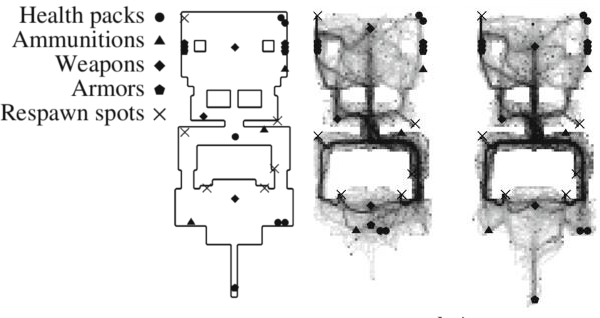
\includegraphics[height=5cm]{d1.png}
\caption{\small{Mappa del livello \texttt{q3dm01} del gioco Quake 3, le ultime due immagini sulla destra mostrano di un colore pi\`u scuro i punti che sono stati percorsi pi\`u spesso}}
\label{img:quake}
\end{figure}

Nella mappa sono rappresentate di un colore differente le zone che sono state maggiormente percorse: si pu\`o notare come alcune zone, in particolare quelle che non contengono oggetti di interesse, siano state maggiormente trascurate rispetto alle zone in prossimit\`a di armi e power-up.

Le misurazioni cambiano drasticamente se si spostano gli oggetti all'interno della mappa (si veda il corridoio nella parte bassa della mappa).

Inoltre si pu\`o notare come siano presenti dei percorsi fissi, che i giocatori percorrono per arrivare prima al power-up desiderato, oppure per raggiungere punti importanti della mappa (colline, o zone in cui si ha una maggiore visibilit\`a e quindi una maggiore probabilit\`a di vittoria).

I risultati delle misurazioni possono quindi essere riassunti nei punti seguenti:

\begin{itemize}
\item I personaggi sono attratti dagli oggetti del gioco, in modo proporzionale alla loro potenzialit\`a ed in particolare se ne hanno urgente bisogno (si pensi ad un medikit).
\item I personaggi sono attratti da altri personaggi che sono amichevoli nei loro confronti (compagni di squadra, altri personaggi con cui commerciare, etc...)
\item I personaggi sono attratti da altri personaggi che risultano indifesi (si nota infatti che un personaggio che inizia a sparare ad un altro personaggio che risulta indifeso tende ad avvicinasi e ad inseguirlo)
\item I personaggi sono attratti da luoghi interessanti (anche detti punti di interesse - POI o \emph{hot-spot)} che possono aiutarli nell'esito della partita: quali colline, torri, avamposti, etc...
\item I personaggi tendono ad allontanarsi da altri personaggi che abbiano un comportamento offensivo nei propri confronti, tendono infatti ad arretrare per evitare di ricevere ulteriori colpi e possono infine scappare
\item I personaggi tendono ad allontanarsi dai luoghi che gli possono arrecare un danno e tendono ad evitare anche le zone in loro prossimita, quali ad esempio pozze di acido, di lava, oppure torri o altre armi che fanno parte della mappa e danneggiano i giocatori.
\end{itemize}

Si noti che molte informazioni sulle relazioni fra i personaggi possono essere raccolte dalla storia stessa dei personaggi: se il personaggio A ha ucciso molte volte il personaggio B e non ha mai ucciso il personaggio C ne risulter\`a che A sar\`a pi\`u attratto da B piuttosto che da C (permettendogli di effettuare pi\`u probabilmente un uccisione) e B tender\`a a scappare da A con una probabilit\`a maggiore rispetto a quella con cui C tender\`a a scappare da A.

Partendo da questi risultati ogni entit\`a genera una quantit\`a di \emph{feromoni} proporzionale alla sua appetibilit\`a.

\subsection{Modello Analitico}

Nel modello \emph{AntDeadReckoning} il mondo \`e diviso in celle di eguale grandezza, ogni cella contiene un certo numero di feromoni che esercitano una certa attrattiva verso i propri vicini.

Per ogni personaggio si definisce una \emph{attraction region} ovvero una regione prossima al personaggio in cui le caselle contenente feromoni vengono considerate per calcolare la forza risultante sul personaggio.

Utilizzando questo modello si pu\`o calcolare la posizione come:
$$ \bm{x}(t) = \bm{x}(0) + \bm{v}(0)\cdot t + \frac{1}{2} \left( \alpha \cdot \frac{1}{m} \bm{F} + (1 - \alpha) \cdot \bm{a}(0) \right) t^2 $$

Dove $\bm{F}$ rappresenta la somma vettoriale delle forze attrattive esercitate dai feromoni presenti nelle celle dell'\emph{attraction region}. Il parametro $\alpha$ varia da 0 a 1 e permette di far pesare la predizione fra l'accelerazione e l'attrazione generata dai feromoni vicini. Il termine $\bm{F}$ risulta essere diviso per la massa del personaggio $m$ in ottemperanza alla formula fisica di Newton $\bm{F} = m \cdot \bm{a}$.

La forza viene calcolata come un vettore centrato nel personaggi, avente come direzione la retta passante fra il personaggio e la cella contenente i feromoni, e ha modulo direttamente proporzionale alla quantit\`a di feromoni e inversamente proporzionale alla distanza (immagine \ref{img:ant}).

$$|| \bm{f}_t (cell, x_t) || = \frac{\textrm{ph}_t (cell)}{d(cell, x_t)^k} $$

Dove $\textrm{ph}_t (cell)$ rappresenta la quantit\`a di feromoni al tempo $t$ e $d(cell, x_t)$ rappresenta la distanza fra la cella e la posizione di $x_t$ e $k$ \`e un parametro del sistema.

Nel caso di entit\`a che si respingono ovviamente il modulo \`e negativo.

\begin{figure}[ht]
\centering
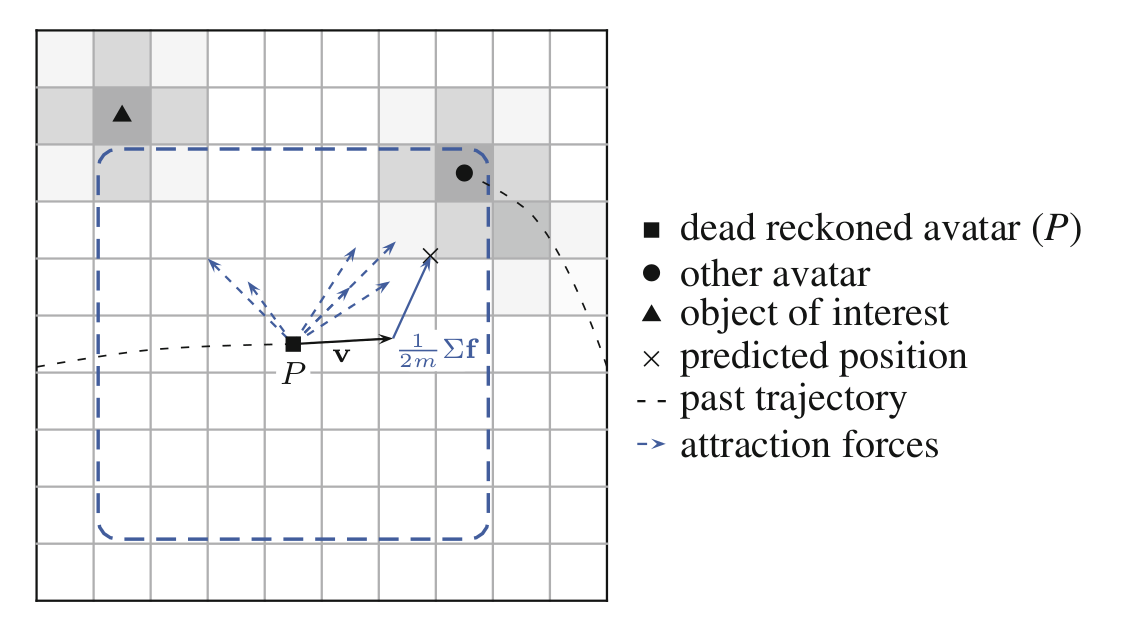
\includegraphics[height=5cm]{d2.png}
\caption{\small{Esempio di \emph{AntDeadReckoning}, con \emph{attraction region} e vettori che rappresentano le forze esercitate dalle caselle contenenti feromoni.}}
\label{img:ant}
\end{figure}


\subsection{Dinamica dei Feromoni}

Il numero di feromoni che sono presenti in una cella non \`e statico, ma varia nel tempo in base ad una serie di fenomeni:

\begin{description}
\item[Generation] Ogni entit\`a presente in una cella genera un numero di feromoni proporzionale alla sua appetitibilit\`a nei confronti del giocatore P. \`E possibile definire un valore $(\textrm{ph}_{max})$ come valore massimo dei feromoni presente in una casella in modo da limitarne l'aumento;
\item[Evaporation] I feromoni presenti in un cella diminuiscono (``evaporano'') rispetto a quelli presenti nel passato in base ad un parametro $\varepsilon$ compreso fra 0 ed 1: $\varepsilon = 0$ sta ad indicare che i feromoni vengono dispersi immediatamente, $\varepsilon = 1$ sta ad indicare che i feromoni non si disperdono mai;
\item[Dissemination] I feromoni si spostano fra caselle adiacenti in base ad una velocit\`a e vengono rallentati da muri ed altri ostacoli, in modo da modellare il fatto che i personaggi non passeranno attraverso muri ed ostacoli.
\end{description}

Questi fenomeni vengono sintetizzati nella formula seguente che rappresenta la quantit\`a di feromoni in un casella $cell$ al tempo $t$ per il giocatore $P$.

\begin{equation}
\begin{split}
\textrm{ph}_t (\textrm{cell}) = \overbrace{\varepsilon \cdot \textrm{ph}_{t-1} (\textrm{cell})}^{\text{Evaporation}} + \overbrace{\sum_{\textrm{ent} \in \textrm{cell}} \textrm{attract}(\textrm{ent}, P)}^{\text{Generation}} + \\ + \underbrace{\sum_{c \in N(\text{cell})} \frac{\varepsilon \cdot \gamma}{N(c)} \cdot \textrm{ph}_{t-1} (\textrm{c})}_{\text{In Dissemination}} - \underbrace{\varepsilon \cdot \gamma \textrm{ph}_{t-1} (\text{cell})}_{\text{Out Dissemination}}
\end{split}
\end{equation}

Dove $\text{attract}$ \`e una funzione che rappresenta l'attrattivit\`a di ogni entit\`a presente nella cella nei confronti del personaggio P, $N(\text{cell})$ rappresenta i vicini della cella ($\text{cell}$) dove avviene la dissemination, e $\gamma$ \`e un parametro tra 0 ed 1 indicante la percentuale di feromoni che vengono disseminati fra i vicini (dopo che parte dei feromoni sono evaporati, per questo \`e moltiplicato per $\varepsilon$).

%\section{Esempio di \emph{Dead Reckoning}}
%
%Nell'esempio che segue si prova a valutare gli effetti del \emph{Dead Reckoning} su un'esperienza di gioco reale. In particolare il gioco in questione \`e \emph{League of Legends}, che implementa la funzione di predizione della posizione (attivabile dalle impostazioni di gioco).
%
%Per simulare un delay di rete \`e stata utilizzato una client che si connette tramite una connessione wireless, inoltre \`e stata saturata la banda avviando un client Bittorrent sulla stessa macchina in modo che i pacchetti ricevuti avessero un ping di circa $600 \text{msec}$.
%
%Il video della simulazione \`e presente all'indirizzo \url{http://ncorti.it/p2p_lol.mp4}: nel video si vede chiaramente come l'avatar del client non affetto da ritardi (avatar \textbf{A}) effettua una traiettoria passante lungo i funghi, mentre il client affetto da ritardi percepisca una traiettoria approssimata.
%
%\begin{figure}[ht]
%\centering
%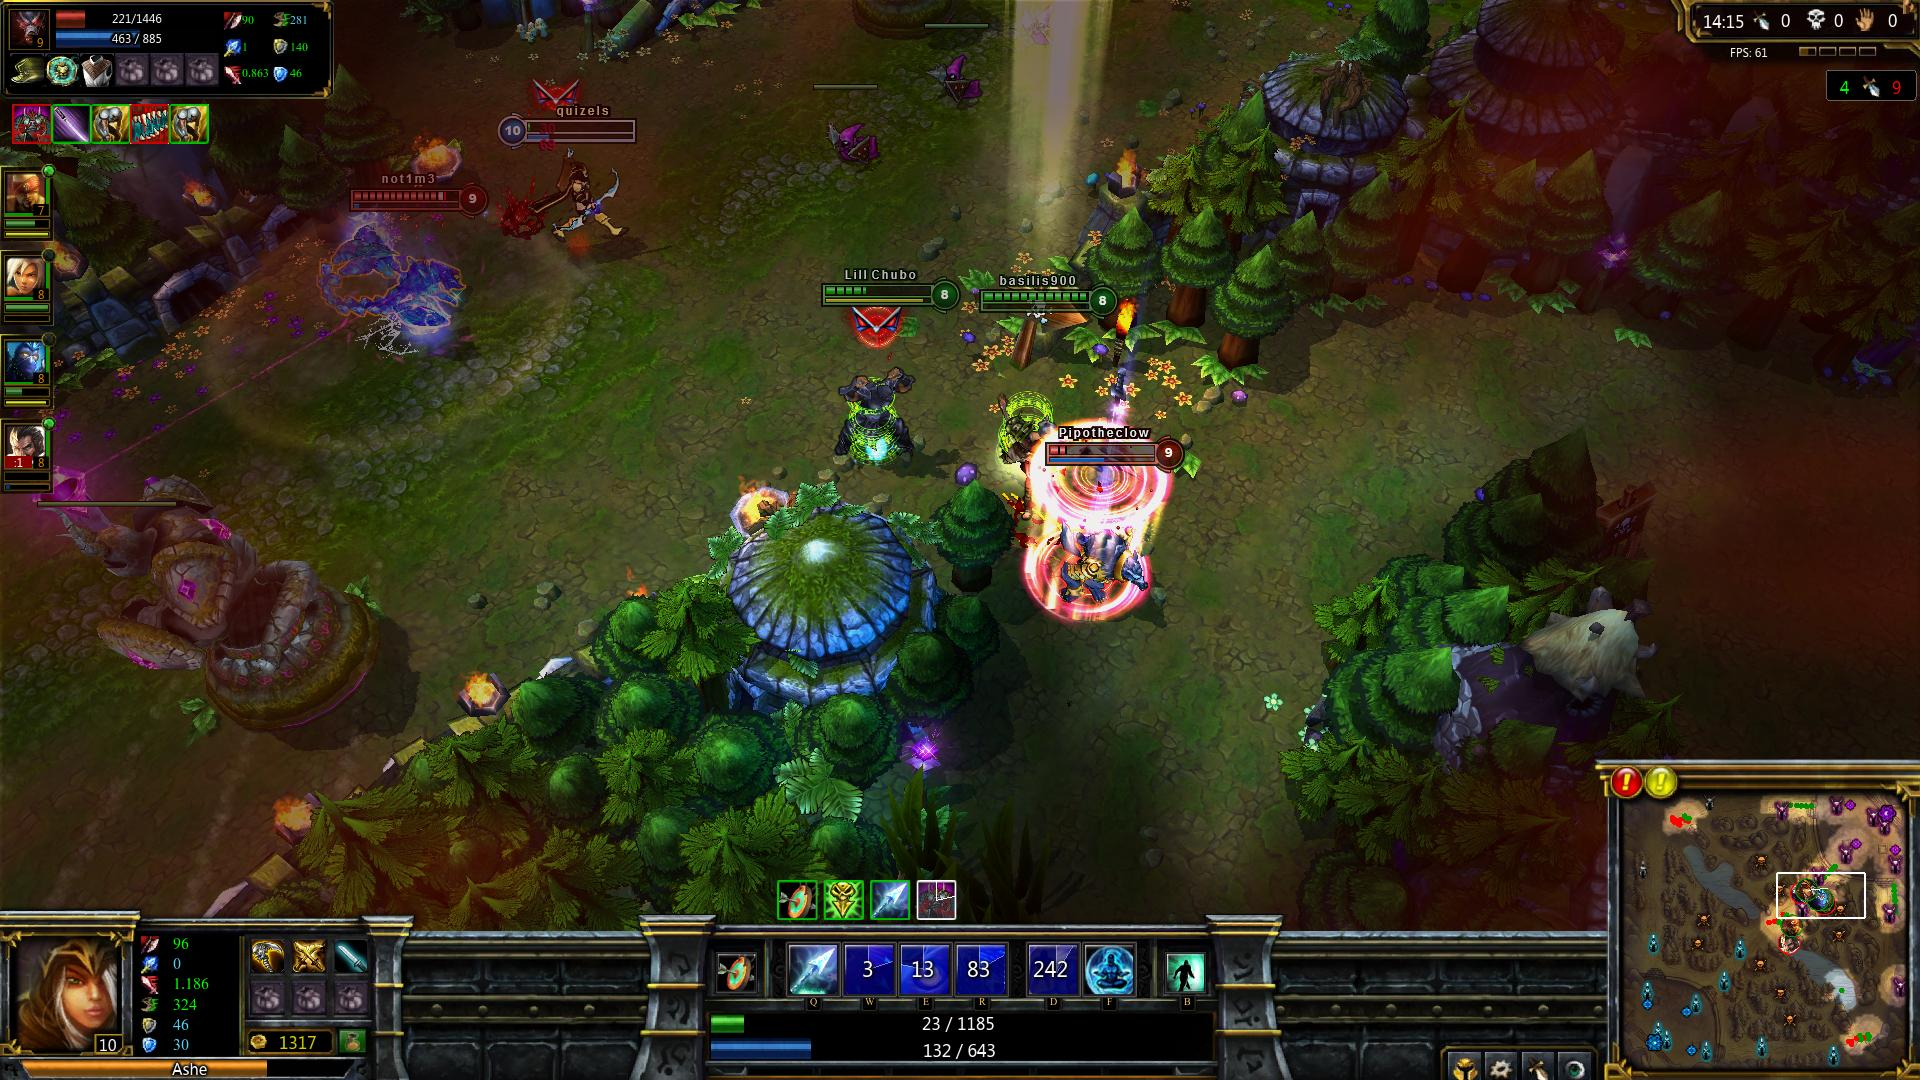
\includegraphics[height=7cm]{lol.jpg}
%\caption{\small{Screenshot del video contenente la simulazione del gioco \emph{League of Legends}}}
%\label{img:lol}
%\end{figure}

\begin{thebibliography}{100}

\bibitem{wiki1} \small{\url{http://en.wikipedia.org/wiki/History_of_massively_multiplayer_online_games} } - Wikipedia

\bibitem{rif1} Smed, J., Hakonen H., \emph{University of Tarku, Finland} (2006). Algorithms and Networking
for Computer Games. \emph{Wiley} (191-195 pp.)  

\bibitem{wiki2} \url{http://en.wikipedia.org/wiki/Lag_(online_gaming)} - Wikipedia

\bibitem{rif2} Pantel, L. \& Wolf, L. C., (2002, April) On the suitability of dead reckoning schemes for games. In \emph{Proceedings of the 1st workshop on Network and system support for games} (79-84 pp.). ACM.

\bibitem{rif3} Aggarwal, S., Banavar, H., Khandelwal, A., Mukherjee, S., \& Rangarajan, S. (2004, August). Accuracy in dead-reckoning based distributed multi-player games. In \emph{Proceedings of 3rd ACM SIGCOMM workshop on Network and system support for games} (161-165 pp.). ACM.

\bibitem{rif4} Mauve, M. (2000, January). How to keep a dead man from shooting. In \emph{Interactive Distributed Multimedia Systems and Telecommunication Services} (199-204 pp.). Springer Berlin Heidelberg.

\bibitem{rif5} Yahyavi, A., Huguenin, K., \& Kemme, B. (June 2013). Interest modeling in games: the case of dead reckoning. \emph{Multimedia Systems}  (Volume 19, Issue 3, 255-270 pp.).

\end{thebibliography}

\end{document}